\documentclass[11pt]{article}
\usepackage[margin=18mm,headheight=22pt]{geometry}
\usepackage{amsmath}
\usepackage{fontspec}
\usepackage{unicode-math}
\setmainfont{NewCM10}[Extension=.otf,UprightFont=*-Book,BoldFont=*-Bold,ItalicFont=*-BookItalic,BoldItalicFont=*-BoldItalic]
\setsansfont{NewCMSans10}[Extension=.otf,UprightFont=*-Book,BoldFont=*-Bold,ItalicFont=*-BookOblique,BoldItalicFont=*-BoldOblique]
\setmathfont{NewCMMath-Book.otf}
\usepackage{xcolor}
\definecolor{FAUblue}{HTML}{04316A}
\definecolor{Paperblue}{HTML}{EEF2F7}
\definecolor{EEIgold}{HTML}{CC9C42}
\usepackage{etoolbox,enumitem,booktabs,tabularx,array,needspace,microtype}
\usepackage[most]{tcolorbox}
\usepackage{titlesec,fancyhdr}
\usepackage[hidelinks]{hyperref}
\usepackage{draftwatermark}
\SetWatermarkText{Made by Thanate Amornjiraporn (Focus)}
\SetWatermarkColor{black!7}\SetWatermarkFontSize{30pt}\SetWatermarkAngle{45}
\setlength{\parindent}{0pt}
\setlength{\parskip}{5pt}
\setlist{itemsep=2pt,topsep=3pt,leftmargin=1.6em,beginpenalty=10000,endpenalty=10000}
\raggedbottom
\clubpenalty=10000 \widowpenalty=10000 \displaywidowpenalty=10000 \interlinepenalty=10000
\setcounter{secnumdepth}{0}
\setcounter{tocdepth}{1}
\pagestyle{fancy}\fancyhf{}
\fancyhead[L]{\small\sffamily\color{FAUblue} From Fundamentals to AI Apocalypse · MEI · Exercise Sheet 3}
\fancyhead[R]{\small\sffamily Exercise 3: Worked solutions}
\fancyfoot[C]{\small\thepage}
\titleformat{\section}{\Large\bfseries\sffamily\color{FAUblue}}{}{0pt}{}
\titleformat{\subsection}{\large\bfseries\sffamily\color{FAUblue}}{}{0pt}{}
\titlespacing*{\section}{0pt}{16pt}{6pt}
\preto\section{\Needspace{8\baselineskip}}
\preto\subsection{\Needspace{6\baselineskip}}
\newtcolorbox{equationcard}[1]{colback=Paperblue,colframe=Paperblue,boxrule=0pt,arc=0pt,left=10pt,right=10pt,top=6pt,bottom=6pt,title={#1},fonttitle=\small\bfseries\sffamily,coltitle=FAUblue,before skip=8pt,after skip=8pt}
\newtcolorbox{workedbox}[1]{colback=white,colframe=EEIgold,boxrule=0pt,leftrule=3pt,arc=0pt,left=10pt,top=4pt,bottom=4pt,title={#1},fonttitle=\small\bfseries\sffamily,coltitle=FAUblue,attach title to upper={\par},before skip=8pt,after skip=8pt}
\newtcolorbox{recallbox}[1]{colback=white,colframe=FAUblue,boxrule=0pt,leftrule=3pt,arc=0pt,left=10pt,top=4pt,bottom=4pt,title={#1},fonttitle=\small\bfseries\sffamily,coltitle=FAUblue,attach title to upper={\par},before skip=8pt,after skip=8pt}
\usepackage{environ}
\newsavebox\measurebox
% Typeset the section once invisibly to measure it; start a new page if it will not fit in what is left.
\makeatletter
\newif\ifkeep@measuring
\NewEnviron{keepsection}{%
  \ifkeep@measuring \BODY \else
    \edef\keep@sec{\the\value{section}}\edef\keep@sub{\the\value{subsection}}%
    \setbox\measurebox\vbox{\hsize\linewidth\keep@measuringtrue\def\Needspace##1{}\BODY}%
    \setcounter{section}{\keep@sec}\setcounter{subsection}{\keep@sub}%
    \dimen2=\ht\measurebox \advance\dimen2\dp\measurebox
    \dimen@=\textheight
    \ifdim\pagegoal<\maxdimen
      \dimen@=\pagegoal \advance\dimen@-\pagetotal
      \ifdim\dimen2>\dimen@ \clearpage \dimen@=\textheight \fi
    \fi
    % if it fits, nothing inside may force an early break
    \ifdim\dimen2>\dimen@ \BODY \else \begingroup\def\Needspace##1{}\BODY\endgroup \fi
  \fi}
\makeatother
\newtcolorbox{notebox}{colback=Paperblue,colframe=Paperblue,boxrule=0pt,arc=0pt,left=8pt,right=8pt,top=4pt,bottom=4pt,before skip=6pt,after skip=6pt}
\newtcolorbox{plainbox}{colback=white,colframe=FAUblue,boxrule=0pt,leftrule=3pt,arc=0pt,left=10pt,right=8pt,top=4pt,bottom=4pt,before skip=6pt,after skip=8pt}
\usetikzlibrary{arrows.meta}
\title{\sffamily\bfseries\color{FAUblue}Exercise 3: Worked solutions}
\author{Mathematics for Engineers I \ensuremath{\cdot} Module 62765 \ensuremath{\cdot} Exercise Sheet 3\\[2pt]\small From Fundamentals to AI Apocalypse · personal study guide}
\date{}
\begin{document}
\maketitle
\begingroup\footnotesize\setlength{\parskip}{0pt}\tableofcontents\endgroup
\clearpage

\begin{keepsection}
\Needspace{9\baselineskip}
\section{Exercise 3.1: Mathematical induction}

\Needspace{6\baselineskip}
Induction separates an infinite claim into a base case and a step showing each case implies the next.

\textbf{Connected topic:} Mathematical induction (§2.5) gives the two-part proof structure used in both claims.

\begin{keepsection}
\Needspace{7\baselineskip}
\subsection{1a: Prove the square-sum inequality}

\Needspace{4\baselineskip}
Try first: write the base case, then add the new final term (n + 1)\textsuperscript{2} to the induction hypothesis.

\nopagebreak[4]{\small\itshape Answers: see “Exercise 3.1: Mathematical induction” under Answers at the end.}
\end{keepsection}

\begin{keepsection}
\Needspace{6\baselineskip}
\subsection{1b: Prove 4 divides 5\textsuperscript{n} \ensuremath{-} 1}

\Needspace{3\baselineskip}
Try first: check n = 1 and rewrite the next power using 5\ensuremath{\cdot}5\textsuperscript{n}.

\nopagebreak[4]{\small\itshape Answers: see “Exercise 3.1: Mathematical induction” under Answers at the end.}
\end{keepsection}
\end{keepsection}

\begin{keepsection}
\Needspace{8\baselineskip}
\section{Exercise 3.2: Maps}

\Needspace{5\baselineskip}
Injectivity asks whether different inputs can share an output; surjectivity asks whether every target value is reached. A bijection has both properties.

\textbf{Connected topics:} Types of mappings (§3.2), inverse functions (§3.3), and composition (§3.4).

\begin{keepsection}
\Needspace{7\baselineskip}
\subsection{2a: Classify f(x) = e\textsuperscript{\ensuremath{-}x\textsuperscript{2}} and g(x,y) = (4y,x\ensuremath{-}1)}

\Needspace{4\baselineskip}
Try first: find the range and look for two different inputs with the same output; for g, solve its two coordinate equations.

\nopagebreak[4]{\small\itshape Answers: see “Exercise 3.2: Maps” under Answers at the end.}

\Needspace{14\baselineskip}
\begin{center}
\begin{minipage}[t]{0.950\linewidth}\centering
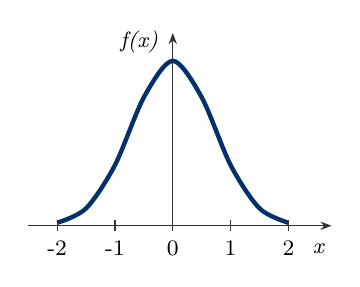
\begin{tikzpicture}[line join=round]
\draw[-{Stealth[length=4pt]},black!80] (0.720,-2.628) -- (4.572,-2.628);
\draw[-{Stealth[length=4pt]},black!80] (2.556,-2.628) -- (2.556,-0.180);
\draw[FAUblue,line width=1.6pt] plot[smooth,tension=0.5] coordinates {(1.087,-2.590) (1.454,-2.408) (1.822,-1.857) (2.189,-0.996) (2.556,-0.533) (2.923,-0.996) (3.290,-1.857) (3.658,-2.408) (4.025,-2.590)};
\node[anchor=east,inner sep=1pt,font=\footnotesize] at (4.536,-2.916) {\textit{x}};
\node[anchor=east,inner sep=1pt,font=\footnotesize] at (2.412,-0.288) {\textit{f(x)}};
\draw[black!80] (1.087,-2.556) -- (1.087,-2.700);
\node[,inner sep=1pt,font=\footnotesize] at (1.087,-2.916) {-2};
\draw[black!80] (1.822,-2.556) -- (1.822,-2.700);
\node[,inner sep=1pt,font=\footnotesize] at (1.822,-2.916) {-1};
\draw[black!80] (2.556,-2.556) -- (2.556,-2.700);
\node[,inner sep=1pt,font=\footnotesize] at (2.556,-2.916) {0};
\draw[black!80] (3.290,-2.556) -- (3.290,-2.700);
\node[,inner sep=1pt,font=\footnotesize] at (3.290,-2.916) {1};
\draw[black!80] (4.025,-2.556) -- (4.025,-2.700);
\node[,inner sep=1pt,font=\footnotesize] at (4.025,-2.916) {2};
\end{tikzpicture}\par\smallskip{\small\raggedright \textbf{f(x) = e\textsuperscript{\ensuremath{-}x\textsuperscript{2}}.} The even graph shows why f(x) = f(\ensuremath{-}x); its values stay positive and at most 1.\par}\end{minipage}
\end{center}
\end{keepsection}

\begin{keepsection}
\Needspace{7\baselineskip}
\subsection{2b(i): Decide whether f \ensuremath{\circ} g can be formed}

\Needspace{4\baselineskip}
Try first: compare the output type of the inner map g with the input type required by the outer map f.

\nopagebreak[4]{\small\itshape Answers: see “Exercise 3.2: Maps” under Answers at the end.}
\end{keepsection}

\begin{keepsection}
\Needspace{6\baselineskip}
\subsection{2b(ii): Find f \ensuremath{\circ} f}

\Needspace{3\baselineskip}
Try first: substitute f(x) into the outer f and simplify the square in the exponent.

\nopagebreak[4]{\small\itshape Answers: see “Exercise 3.2: Maps” under Answers at the end.}
\end{keepsection}

\begin{keepsection}
\Needspace{6\baselineskip}
\subsection{2b(iii): Find g \ensuremath{\circ} g}

\Needspace{3\baselineskip}
Try first: substitute (4y,x\ensuremath{-}1) for the input pair of the outer g.

\nopagebreak[4]{\small\itshape Answers: see “Exercise 3.2: Maps” under Answers at the end.}
\end{keepsection}
\end{keepsection}

\begin{keepsection}
\Needspace{7\baselineskip}
\section{Exercise 3.3: Properties of the binomial coefficient}

\Needspace{4\baselineskip}
All three identities follow from the factorial definition; the last is Pascal’s rule.

\textbf{Connected topic:} Binomial coefficients (§2.4) introduces factorials and Pascal’s identity.

\begin{keepsection}
\Needspace{6\baselineskip}
\subsection{3i: Prove C(n,n) = C(n,0) = 1}

\Needspace{3\baselineskip}
Try first: substitute k = n and k = 0 into the factorial definition, using 0! = 1.

\nopagebreak[4]{\small\itshape Answers: see “Exercise 3.3: Properties of the binomial coefficient” under Answers at the end.}
\end{keepsection}

\begin{keepsection}
\Needspace{6\baselineskip}
\subsection{3ii: Prove C(n,k) = C(n,n\ensuremath{-}k)}

\Needspace{3\baselineskip}
Try first: write both sides using factorials and compare the denominator factors.

\nopagebreak[4]{\small\itshape Answers: see “Exercise 3.3: Properties of the binomial coefficient” under Answers at the end.}
\end{keepsection}

\begin{keepsection}
\Needspace{6\baselineskip}
\subsection{3iii: Prove Pascal’s identity}

\Needspace{3\baselineskip}
Try first: put the two left-hand fractions over the common denominator (k+1)!(n\ensuremath{-}k)!.

\nopagebreak[4]{\small\itshape Answers: see “Exercise 3.3: Properties of the binomial coefficient” under Answers at the end.}
\end{keepsection}
\end{keepsection}

\begin{keepsection}
\Needspace{9\baselineskip}
\section{Exercise 3.4: Elementary functions}

\Needspace{6\baselineskip}
Substituting x\textsuperscript{4} reduces the degree-eight polynomial to a quadratic. The number of real roots of the parameterized quadratic is controlled by its discriminant.

\textbf{Connected topics:} Elementary functions (§3.5) and the quadratic formula and inequalities (§2.3).

\begin{keepsection}
\Needspace{7\baselineskip}
\subsection{4a: Find and factor the real roots of f(x) = x\textsuperscript{8} \ensuremath{-} 3x\textsuperscript{4} \ensuremath{-} 4}

\Needspace{4\baselineskip}
Try first: set t = x\textsuperscript{4}. Remember t cannot be negative, even though the resulting quadratic has two algebraic roots.

\nopagebreak[4]{\small\itshape Answers: see “Exercise 3.4: Elementary functions” under Answers at the end.}
\end{keepsection}

\begin{keepsection}
\Needspace{7\baselineskip}
\subsection{4b: Choose c so g\textsubscript{c}(x) = 3x\textsuperscript{2} + 2x + c has exactly one real root}

\Needspace{4\baselineskip}
Try first: set the discriminant to zero, then find the repeated root and write the factorization.

\nopagebreak[4]{\small\itshape Answers: see “Exercise 3.4: Elementary functions” under Answers at the end.}
\end{keepsection}
\end{keepsection}

\begin{keepsection}
\Needspace{8\baselineskip}
\section{Self-Study 3.5: Mathematical induction}

\Needspace{5\baselineskip}
The finite geometric-sum formula is proved by adding exactly one new power and simplifying over the fixed denominator.

\textbf{Connected topic:} Mathematical induction (§2.5) supplies the base-step method.

\begin{keepsection}
\Needspace{6\baselineskip}
\subsection{5: Prove the finite geometric-sum formula}

\Needspace{3\baselineskip}
Try first: use n = 1 as the base case; in the step, add x\textsuperscript{n+1} to the assumed sum.

\nopagebreak[4]{\small\itshape Answers: see “Self-Study 3.5: Mathematical induction” under Answers at the end.}
\end{keepsection}
\end{keepsection}

\begin{keepsection}
\Needspace{8\baselineskip}
\section{Self-Study 3.6: Power sums}

\Needspace{5\baselineskip}
Each identity is proved independently: the induction step adds the new term (n+1), (n+1)\textsuperscript{2}, or (n+1)\textsuperscript{3} and factors the result.

\textbf{Connected topic:} Induction (§2.5) supports each proof; the sum notation is reviewed in §2.4.

\begin{keepsection}
\Needspace{6\baselineskip}
\subsection{6a: Prove \ensuremath{\Sigma}\textsubscript{k=1}\textsuperscript{n} k = n(n+1)/2}

\Needspace{3\baselineskip}
Try first: check n = 1, then add n+1 to the formula at n.

\nopagebreak[4]{\small\itshape Answers: see “Self-Study 3.6: Power sums” under Answers at the end.}
\end{keepsection}

\begin{keepsection}
\Needspace{6\baselineskip}
\subsection{6b: Prove \ensuremath{\Sigma}\textsubscript{k=1}\textsuperscript{n} k\textsuperscript{2} = n(n+1)(2n+1)/6}

\Needspace{3\baselineskip}
Try first: after adding (n+1)\textsuperscript{2}, factor out n+1 and compare with the target at n+1.

\nopagebreak[4]{\small\itshape Answers: see “Self-Study 3.6: Power sums” under Answers at the end.}
\end{keepsection}

\begin{keepsection}
\Needspace{6\baselineskip}
\subsection{6c: Prove \ensuremath{\Sigma}\textsubscript{k=1}\textsuperscript{n} k\textsuperscript{3} = (n(n+1)/2)\textsuperscript{2}}

\Needspace{3\baselineskip}
Try first: add (n+1)\textsuperscript{3} to the squared induction hypothesis, then factor (n+1)\textsuperscript{2}.

\nopagebreak[4]{\small\itshape Answers: see “Self-Study 3.6: Power sums” under Answers at the end.}
\end{keepsection}
\end{keepsection}

\begin{keepsection}
\Needspace{8\baselineskip}
\section{Self-Study 3.7: Maps}

\Needspace{5\baselineskip}
Vertex form gives the range and symmetry of the quadratic. For compositions, the inner output must lie in the outer function’s domain.

\textbf{Connected topics:} Types of mappings (§3.2), inverse functions (§3.3), and composition (§3.4).

\begin{keepsection}
\Needspace{7\baselineskip}
\subsection{7a: Classify f, g and h}

\Needspace{4\baselineskip}
Try first: write f in vertex form, determine the actual range of g, and solve h(x,y,z)=(u,v) for arbitrary u,v.

\nopagebreak[4]{\small\itshape Answers: see “Self-Study 3.7: Maps” under Answers at the end.}

\Needspace{14\baselineskip}
\begin{center}
\begin{minipage}[t]{0.950\linewidth}\centering
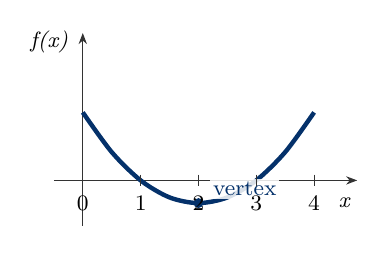
\begin{tikzpicture}[line join=round]
\draw[-{Stealth[length=4pt]},black!80] (0.720,-2.052) -- (4.572,-2.052);
\draw[-{Stealth[length=4pt]},black!80] (1.087,-2.628) -- (1.087,-0.180);
\draw[FAUblue,line width=1.6pt] plot[smooth,tension=0.5] coordinates {(1.087,-1.188) (1.454,-1.692) (1.822,-2.052) (2.189,-2.268) (2.556,-2.340) (2.923,-2.268) (3.290,-2.052) (3.658,-1.692) (4.025,-1.188)};
\fill[FAUblue] (2.556,-2.340) circle (0.063);
\node[anchor=west,text=FAUblue,fill=white,fill opacity=0.85,text opacity=1,inner sep=1pt,font=\footnotesize] at (2.700,-2.160) {vertex};
\node[anchor=east,inner sep=1pt,font=\footnotesize] at (4.536,-2.340) {\textit{x}};
\node[anchor=east,inner sep=1pt,font=\footnotesize] at (0.943,-0.288) {\textit{f(x)}};
\draw[black!80] (1.087,-1.980) -- (1.087,-2.124);
\node[,inner sep=1pt,font=\footnotesize] at (1.087,-2.340) {0};
\draw[black!80] (1.822,-1.980) -- (1.822,-2.124);
\node[,inner sep=1pt,font=\footnotesize] at (1.822,-2.340) {1};
\draw[black!80] (2.556,-1.980) -- (2.556,-2.124);
\node[,inner sep=1pt,font=\footnotesize] at (2.556,-2.340) {2};
\draw[black!80] (3.290,-1.980) -- (3.290,-2.124);
\node[,inner sep=1pt,font=\footnotesize] at (3.290,-2.340) {3};
\draw[black!80] (4.025,-1.980) -- (4.025,-2.124);
\node[,inner sep=1pt,font=\footnotesize] at (4.025,-2.340) {4};
\end{tikzpicture}\par\smallskip{\small\raggedright \textbf{f(x)=(x\ensuremath{-}2)\textsuperscript{2}\ensuremath{-}1.} The symmetry around x=2 explains why f is not injective on all of \ensuremath{\mathbb{R}}; restricting to one side of the vertex makes it invertible.\par}\end{minipage}
\end{center}
\end{keepsection}

\begin{keepsection}
\Needspace{7\baselineskip}
\subsection{7b(i): Form f \ensuremath{\circ} s}

\Needspace{4\baselineskip}
Try first: substitute sin x into f, then find the range by examining the resulting quadratic for t=sin x\ensuremath{\in}[\ensuremath{-}1,1].

\nopagebreak[4]{\small\itshape Answers: see “Self-Study 3.7: Maps” under Answers at the end.}
\end{keepsection}

\begin{keepsection}
\Needspace{6\baselineskip}
\subsection{7b(ii): Form g \ensuremath{\circ} f}

\Needspace{3\baselineskip}
Try first: require f(x)\ensuremath{\leq}1 before substituting it under the square root.

\nopagebreak[4]{\small\itshape Answers: see “Self-Study 3.7: Maps” under Answers at the end.}
\end{keepsection}

\begin{keepsection}
\Needspace{7\baselineskip}
\subsection{7b(iii): Form g \ensuremath{\circ} s}

\Needspace{4\baselineskip}
Try first: check whether every value of sin x lies in g’s domain, then use the extreme sine values for the range.

\nopagebreak[4]{\small\itshape Answers: see “Self-Study 3.7: Maps” under Answers at the end.}
\end{keepsection}

\begin{keepsection}
\Needspace{7\baselineskip}
\subsection{7b(iv): Form g \ensuremath{\circ} g}

\Needspace{4\baselineskip}
Try first: require the output of the inner g to be at most 1, not just that the original x is at most 1.

\nopagebreak[4]{\small\itshape Answers: see “Self-Study 3.7: Maps” under Answers at the end.}
\end{keepsection}
\end{keepsection}

\begin{keepsection}
\Needspace{9\baselineskip}
\section{Self-Study 3.8: Finite decimals and computer arithmetic}

\Needspace{6\baselineskip}
Finite decimals form a set closed under addition and multiplication, but they do not include every rational. Truncation gives controlled approximations; floating-point arithmetic can change familiar algebraic laws.

\textbf{Connected topics:} Number systems (§2.1) and real-number arithmetic (§2.2).

\begin{keepsection}
\Needspace{7\baselineskip}
\subsection{8a: Prove D is closed under addition and multiplication}

\Needspace{4\baselineskip}
Try first: put two denominators over a common power of 10 for the sum; multiply numerators and denominators for the product.

\nopagebreak[4]{\small\itshape Answers: see “Self-Study 3.8: Finite decimals and computer arithmetic” under Answers at the end.}
\end{keepsection}

\begin{keepsection}
\Needspace{6\baselineskip}
\subsection{8b: Prove 1/3 \ensuremath{\notin} D}

\Needspace{3\baselineskip}
Try first: assume 1/3=m/10\textsuperscript{n} and examine the resulting equality modulo 3.

\nopagebreak[4]{\small\itshape Answers: see “Self-Study 3.8: Finite decimals and computer arithmetic” under Answers at the end.}
\end{keepsection}

\begin{keepsection}
\Needspace{7\baselineskip}
\subsection{8c: Prove the truncation bounds}

\Needspace{4\baselineskip}
Try first: apply the defining inequality for floor(10\textsuperscript{n}x), then divide by the positive number 10\textsuperscript{n}.

\nopagebreak[4]{\small\itshape Answers: see “Self-Study 3.8: Finite decimals and computer arithmetic” under Answers at the end.}
\end{keepsection}

\begin{keepsection}
\Needspace{7\baselineskip}
\subsection{8d: Compare the two floating-point sums}

\Needspace{4\baselineskip}
Try first: evaluate the parenthesized operations in order and remember that a double cannot represent every integer near 10\textsuperscript{16}.

\nopagebreak[4]{\small\itshape Answers: see “Self-Study 3.8: Finite decimals and computer arithmetic” under Answers at the end.}
\end{keepsection}
\end{keepsection}

\begin{keepsection}
\Needspace{8\baselineskip}
\section{Self-Study 3.9: Fibonacci numbers in Pascal’s triangle}

\Needspace{5\baselineskip}
The diagonal sums in Pascal’s triangle satisfy the same two-step recurrence as the Fibonacci sequence.

\textbf{Connected topics:} Binomial coefficients and Pascal’s identity (§2.4), and induction (§2.5).

\begin{keepsection}
\Needspace{6\baselineskip}
\subsection{9a: Compute F\textsubscript{1} through F\textsubscript{10}}

\Needspace{3\baselineskip}
Try first: start from F\textsubscript{1}=F\textsubscript{2}=1 and add the previous two values at each step.

\nopagebreak[4]{\small\itshape Answers: see “Self-Study 3.9: Fibonacci numbers in Pascal’s triangle” under Answers at the end.}
\end{keepsection}

\begin{keepsection}
\Needspace{6\baselineskip}
\subsection{9b: List Pascal’s rows 0–7 and compute D\textsubscript{0}–D\textsubscript{7}}

\Needspace{3\baselineskip}
Try first: for each n, add C(n\ensuremath{-}k,k) across k; use the stated zero convention when k\ensuremath{>}n\ensuremath{-}k.

\nopagebreak[4]{\small\itshape Answers: see “Self-Study 3.9: Fibonacci numbers in Pascal’s triangle” under Answers at the end.}
\end{keepsection}

\begin{keepsection}
\Needspace{6\baselineskip}
\subsection{9c: Prove D\textsubscript{n} = F\textsubscript{n+1} by induction}

\Needspace{3\baselineskip}
Try first: derive D\textsubscript{n+2}=D\textsubscript{n+1}+D\textsubscript{n} from Pascal’s identity, then use two initial values.

\nopagebreak[4]{\small\itshape Answers: see “Self-Study 3.9: Fibonacci numbers in Pascal’s triangle” under Answers at the end.}
\end{keepsection}
\end{keepsection}


\clearpage
\section{Answers}
\begin{keepsection}\subsection{Exercise 3.1: Mathematical induction}

\begin{workedbox}{1a \ensuremath{\cdot} Induction on n}
\Needspace{10\baselineskip}
\begin{enumerate}
\item \textbf{Claim:} S\textsubscript{n} = \ensuremath{\textstyle\sum}\textsubscript{k=1}\textsuperscript{n}(k \ensuremath{-} 1)\textsuperscript{2} \ensuremath{<} n\textsuperscript{3}/3.
\item \textbf{Base case n = 1:} S\textsubscript{1} = (1\ensuremath{-}1)\textsuperscript{2} = 0 \ensuremath{<} 1/3, so the claim starts true.
\item \textbf{Induction hypothesis:} assume S\textsubscript{n} \ensuremath{<} n\textsuperscript{3}/3 for some n \ensuremath{\in} \ensuremath{\mathbb{N}}.
\item \Needspace{4\baselineskip}
The next sum adds the term k = n + 1, which equals n\textsuperscript{2}:

\begin{equation*}\mathrm{S}_{\mathrm{n}+1}\, =\, \mathrm{S}_{\mathrm{n}}\, +\, \mathrm{n}^{2}\, <\, \mathrm{n}^{3}/3\, +\, \mathrm{n}^{2}\end{equation*}
\item \Needspace{4\baselineskip}
Compare the upper bound with the target:

\begin{equation*}(\mathrm{n}\, +\, 1)^{3}/3\, =\, \mathrm{n}^{3}/3\, +\, \mathrm{n}^{2}\, +\, \mathrm{n}\, +\, 1/3\, >\, \mathrm{n}^{3}/3\, +\, \mathrm{n}^{2}\end{equation*}
\item Therefore S\textsubscript{n+1} \ensuremath{<} (n + 1)\textsuperscript{3}/3. The base and step prove the claim for every n \ensuremath{\in} \ensuremath{\mathbb{N}}.
\end{enumerate}
\end{workedbox}

\end{keepsection}
\begin{keepsection}\subsection{Exercise 3.1: Mathematical induction}

\begin{workedbox}{1b \ensuremath{\cdot} Preserve divisibility in the induction step}
\Needspace{8\baselineskip}
\begin{enumerate}
\item \textbf{Base case n = 1:} 5\textsuperscript{1} \ensuremath{-} 1 = 4, divisible by 4.
\item \textbf{Induction hypothesis:} suppose 5\textsuperscript{n} \ensuremath{-} 1 = 4q for some integer q.
\item \Needspace{4\baselineskip}
Then the next expression is:

\begin{equation*}5^{\mathrm{n}+1}\, -\, 1\, =\, 5\cdot 5^{\mathrm{n}}\, -\, 1\, =\, 5(5^{\mathrm{n}}\, -\, 1)\, +\, 4\end{equation*}
\item Substitute the hypothesis: 5(4q) + 4 = 4(5q + 1), a multiple of 4. Hence 4 divides 5\textsuperscript{n} \ensuremath{-} 1 for every positive integer n.
\end{enumerate}
\end{workedbox}

\end{keepsection}
\begin{keepsection}\subsection{Exercise 3.2: Maps}

\begin{workedbox}{2a \ensuremath{\cdot} Range and one-to-one tests}
\Needspace{14\baselineskip}
\begin{enumerate}
\item For f, x\textsuperscript{2} \ensuremath{\geq} 0, so \ensuremath{-}x\textsuperscript{2} \ensuremath{\leq} 0 and 0 \ensuremath{<} e\textsuperscript{\ensuremath{-}x\textsuperscript{2}} \ensuremath{\leq} 1. The maximum 1 occurs at x = 0; the value 0 is approached as |x| grows but is never reached. Thus range(f) = (0,1], so f is not onto \ensuremath{\mathbb{R}}.
\item Also f(1) = f(\ensuremath{-}1) = e\textsuperscript{\ensuremath{-}1} with distinct inputs, so f is not injective. Therefore it is not bijective as stated.
\item \Needspace{5\baselineskip}
Restrict its domain to [0,\ensuremath{\infty}) and its range/codomain to (0,1]. On this domain f decreases strictly from 1 toward 0, so the restricted map is bijective. Solve y = e\textsuperscript{\ensuremath{-}x\textsuperscript{2}} with x \ensuremath{\geq} 0:

\Needspace{4\baselineskip}
\begin{equation*}\ln \, \mathrm{y}\, =\, -\mathrm{x}^{2}\, \Rightarrow \, \mathrm{x}\, =\, \sqrt{-\ln \, \mathrm{y}},\, \quad \, 0\, <\, \mathrm{y}\, \leq \, 1\end{equation*}

Its inverse is f\textsuperscript{\ensuremath{-}1}(y) = \ensuremath{\sqrt{-\ln \, \mathrm{y}}}.
\item For g, if g(x\textsubscript{1},y\textsubscript{1}) = g(x\textsubscript{2},y\textsubscript{2}), coordinate equality gives 4y\textsubscript{1} = 4y\textsubscript{2} and x\textsubscript{1}\ensuremath{-}1 = x\textsubscript{2}\ensuremath{-}1, hence both input coordinates agree. So g is injective.
\item \Needspace{5\baselineskip}
Given any target (u,v) \ensuremath{\in} \ensuremath{\mathbb{R}}\textsuperscript{2}, choose x = v + 1 and y = u/4. Then g(x,y) = (u,v), so g is surjective as well. It is bijective, with:

\begin{equation*}\mathrm{g}^{-1}(\mathrm{u},\mathrm{v})\, =\, (\mathrm{v}\, +\, 1,\, \mathrm{u}/4)\end{equation*}
\end{enumerate}
\end{workedbox}

\end{keepsection}
\begin{keepsection}\subsection{Exercise 3.2: Maps}

\begin{workedbox}{2b(i) \ensuremath{\cdot} Match codomain to domain}
\Needspace{6\baselineskip}
\begin{enumerate}
\item g takes a vector in \ensuremath{\mathbb{R}}\textsuperscript{2} and returns a vector in \ensuremath{\mathbb{R}}\textsuperscript{2}. But f expects a real number, an element of \ensuremath{\mathbb{R}}.
\item The codomain \ensuremath{\mathbb{R}}\textsuperscript{2} of g is not contained in the domain \ensuremath{\mathbb{R}} of f. Thus f \ensuremath{\circ} g is \textbf{not defined} with the stated maps.
\end{enumerate}
\end{workedbox}

\end{keepsection}
\begin{keepsection}\subsection{Exercise 3.2: Maps}

\begin{workedbox}{2b(ii) \ensuremath{\cdot} Compose the real-valued map with itself}
\Needspace{7\baselineskip}
\begin{enumerate}
\item \Needspace{5\baselineskip}
The output of f lies in \ensuremath{\mathbb{R}}, so it is a valid input for f. The composition has domain \ensuremath{\mathbb{R}} and mapping rule:

\begin{equation*}(\mathrm{f}\, \circ \, \mathrm{f})(\mathrm{x})\, =\, \mathrm{e}^{-(\mathrm{e}^{-\mathrm{x}^{2}})^{2}}\, =\, \mathrm{e}^{-\mathrm{e}^{-2\mathrm{x}^{2}}}\end{equation*}
\item The inner value t = f(x) ranges over (0,1]. Applying f to such a t gives e\textsuperscript{\ensuremath{-}t\textsuperscript{2}}, which ranges from e\textsuperscript{\ensuremath{-}1} (at t = 1) up toward, but never reaches, 1 (as t approaches 0).
\item Therefore range(f \ensuremath{\circ} f) = [e\textsuperscript{\ensuremath{-}1},1).
\end{enumerate}
\end{workedbox}

\end{keepsection}
\begin{keepsection}\subsection{Exercise 3.2: Maps}

\begin{workedbox}{2b(iii) \ensuremath{\cdot} Compose the plane map}
\Needspace{6\baselineskip}
\begin{enumerate}
\item Both copies of g map \ensuremath{\mathbb{R}}\textsuperscript{2} to \ensuremath{\mathbb{R}}\textsuperscript{2}, so the composition is defined on all of \ensuremath{\mathbb{R}}\textsuperscript{2}.
\item \Needspace{4\baselineskip}
Apply the rule twice:

\begin{equation*}(\mathrm{g}\, \circ \, \mathrm{g})(\mathrm{x},\mathrm{y})\, =\, \mathrm{g}(4\mathrm{y},\mathrm{x}-1)\, =\, (4(\mathrm{x}-1),4\mathrm{y}-1)\end{equation*}
\item The result is an invertible affine map, so its range is \ensuremath{\mathbb{R}}\textsuperscript{2}. Explicitly, any target (u,v) comes from x = u/4 + 1 and y = (v+1)/4.
\end{enumerate}
\end{workedbox}

\end{keepsection}
\begin{keepsection}\subsection{Exercise 3.3: Properties of the binomial coefficient}

\begin{workedbox}{3i \ensuremath{\cdot} The two endpoint choices}
\Needspace{5\baselineskip}
\begin{enumerate}
\item \Needspace{4\baselineskip}
By definition C(n,k) = n!/[k!(n\ensuremath{-}k)!]. At k = n:

\begin{equation*}\mathrm{C}(\mathrm{n},\mathrm{n})\, =\, \mathrm{n}!/(\mathrm{n}!\cdot 0!)\, =\, 1\end{equation*}
\item \Needspace{4\baselineskip}
At k = 0:

\begin{equation*}\mathrm{C}(\mathrm{n},0)\, =\, \mathrm{n}!/(0!\cdot \mathrm{n}!)\, =\, 1\end{equation*}
\item Each coefficient counts the unique way to choose either all n objects or none.
\end{enumerate}
\end{workedbox}

\end{keepsection}
\begin{keepsection}\subsection{Exercise 3.3: Properties of the binomial coefficient}

\begin{workedbox}{3ii \ensuremath{\cdot} Symmetry under exchanging chosen and omitted objects}
\Needspace{6\baselineskip}
\begin{enumerate}
\item \Needspace{4\baselineskip}
For 0 \ensuremath{\leq} k \ensuremath{\leq} n:

\begin{equation*}\mathrm{C}(\mathrm{n},\mathrm{n}-\mathrm{k})\, =\, \mathrm{n}!/((\mathrm{n}-\mathrm{k})!\cdot (\mathrm{n}-(\mathrm{n}-\mathrm{k}))!)\, =\, \mathrm{n}!/((\mathrm{n}-\mathrm{k})!\cdot \mathrm{k}!)\end{equation*}
\item Factorial multiplication is commutative, so this denominator equals k!(n\ensuremath{-}k)!. That is C(n,k), proving the identity.
\item Combinatorially, choosing k objects is equivalent to choosing the n\ensuremath{-}k objects left behind.
\end{enumerate}
\end{workedbox}

\end{keepsection}
\begin{keepsection}\subsection{Exercise 3.3: Properties of the binomial coefficient}

\begin{workedbox}{3iii \ensuremath{\cdot} Add adjacent binomial coefficients}
\Needspace{8\baselineskip}
\begin{enumerate}
\item \Needspace{4\baselineskip}
Using the factorial definition, the left side is:

\begin{equation*}\mathrm{C}(\mathrm{n},\mathrm{k})\, +\, \mathrm{C}(\mathrm{n},\mathrm{k}+1)\, =\, \mathrm{n}!/[\mathrm{k}!(\mathrm{n}-\mathrm{k})!]\, +\, \mathrm{n}!/[(\mathrm{k}+1)!(\mathrm{n}-\mathrm{k}-1)!]\end{equation*}
\item \Needspace{4\baselineskip}
Use the common denominator (k+1)!(n\ensuremath{-}k)!:

\begin{equation*}=\, ((\mathrm{k}+1)\mathrm{n}!\, +\, (\mathrm{n}-\mathrm{k})\mathrm{n}!)/((\mathrm{k}+1)!(\mathrm{n}-\mathrm{k})!)\, =\, (\mathrm{n}+1)!/((\mathrm{k}+1)!(\mathrm{n}-\mathrm{k})!)\end{equation*}
\item The final fraction is C(n+1,k+1). The stated range 0 \ensuremath{\leq} k \ensuremath{\leq} n\ensuremath{-}1 ensures all factorials above have non-negative integer arguments.
\end{enumerate}
\end{workedbox}

\end{keepsection}
\begin{keepsection}\subsection{Exercise 3.4: Elementary functions}

\begin{workedbox}{4a \ensuremath{\cdot} Reduce to a quadratic in x\textsuperscript{4}}
\Needspace{9\baselineskip}
\begin{enumerate}
\item Let t = x\textsuperscript{4} \ensuremath{\geq} 0. Then f(x) = t\textsuperscript{2} \ensuremath{-} 3t \ensuremath{-} 4 factors as (t\ensuremath{-}4)(t+1).
\item Setting f(x) = 0 gives t = 4 or t = \ensuremath{-}1. The second value is impossible because t = x\textsuperscript{4} \ensuremath{\geq} 0.
\item Thus x\textsuperscript{4} = 4. Equivalently x\textsuperscript{2} = 2, so the real roots are x = \ensuremath{\sqrt{2}} and x = \ensuremath{-}\ensuremath{\sqrt{2}}.
\item \Needspace{4\baselineskip}
Factor fully over \ensuremath{\mathbb{R}}:

\begin{equation*}\mathrm{x}^{8}\, -\, 3\mathrm{x}^{4}\, -\, 4\, =\, (\mathrm{x}-\sqrt{2})(\mathrm{x}+\sqrt{2})(\mathrm{x}^{2}+2)(\mathrm{x}^{2}+\sqrt{2}\mathrm{x}+1)(\mathrm{x}^{2}-\sqrt{2}\mathrm{x}+1)\end{equation*}
\item The remaining quadratics have no real roots: x\textsuperscript{2}+2 is always positive, and each x\textsuperscript{2} \ensuremath{\pm} \ensuremath{\sqrt{2}}x + 1 has discriminant 2\ensuremath{-}4 = \ensuremath{-}2. So the two displayed linear factors are all the real linear factors.
\end{enumerate}
\end{workedbox}

\end{keepsection}
\begin{keepsection}\subsection{Exercise 3.4: Elementary functions}

\begin{workedbox}{4b \ensuremath{\cdot} One distinct root means a repeated root}
\Needspace{9\baselineskip}
\begin{enumerate}
\item For ax\textsuperscript{2}+bx+c the discriminant is b\textsuperscript{2}\ensuremath{-}4ac. Here a = 3 and b = 2, so Δ = 4\ensuremath{-}12c.
\item A real quadratic with non-zero leading coefficient has exactly one distinct real root precisely when Δ = 0. Therefore 4\ensuremath{-}12c = 0, giving c = 1/3.
\item \Needspace{4\baselineskip}
The repeated root is \ensuremath{-}b/(2a) = \ensuremath{-}2/6 = \ensuremath{-}1/3. The corresponding factorization is:

\begin{equation*}\mathrm{g}_{1/3}(\mathrm{x})\, =\, 3\mathrm{x}^{2}\, +\, 2\mathrm{x}\, +\, 1/3\, =\, 3(\mathrm{x}\, +\, 1/3)^{2}\end{equation*}
\item \textbf{Check:} expanding gives 3x\textsuperscript{2}+2x+1/3, and its only distinct root is \ensuremath{-}1/3 (with multiplicity two).
\end{enumerate}
\end{workedbox}

\end{keepsection}
\begin{keepsection}\subsection{Self-Study 3.5: Mathematical induction}

\begin{workedbox}{5 \ensuremath{\cdot} Induction for every x \ensuremath{\neq} 1}
\Needspace{9\baselineskip}
\begin{enumerate}
\item Fix any real x \ensuremath{\neq} 1. The claim is \ensuremath{\Sigma}\textsubscript{k=0}\textsuperscript{n}x\textsuperscript{k} = (1\ensuremath{-}x\textsuperscript{n+1})/(1\ensuremath{-}x).
\item \textbf{Base n = 1:} 1+x = (1\ensuremath{-}x\textsuperscript{2})/(1\ensuremath{-}x), since 1\ensuremath{-}x\textsuperscript{2} = (1\ensuremath{-}x)(1+x).
\item \Needspace{4\baselineskip}
\textbf{Induction hypothesis:} suppose the formula holds for n. Add the next term:

\begin{equation*}\sum_{\mathrm{k}=0}^{\mathrm{n}+1}\mathrm{x}^{\mathrm{k}}\, =\, (1-\mathrm{x}^{\mathrm{n}+1})/(1-\mathrm{x})\, +\, \mathrm{x}^{\mathrm{n}+1}\end{equation*}
\item \Needspace{4\baselineskip}
Put the terms over one denominator and simplify:

\begin{equation*}=\, (1-\mathrm{x}^{\mathrm{n}+1}\, +\, \mathrm{x}^{\mathrm{n}+1}(1-\mathrm{x}))/(1-\mathrm{x})\, =\, (1-\mathrm{x}^{\mathrm{n}+2})/(1-\mathrm{x})\end{equation*}
\item This is the desired formula at n+1. Thus it holds for every n \ensuremath{\in} \ensuremath{\mathbb{N}} and each fixed x \ensuremath{\in} \ensuremath{\mathbb{R}}\textbackslash{}\{1\}.
\end{enumerate}
\end{workedbox}

\end{keepsection}
\begin{keepsection}\subsection{Self-Study 3.6: Power sums}

\begin{workedbox}{6a \ensuremath{\cdot} Sum of the first n integers}
\Needspace{5\baselineskip}
\begin{enumerate}
\item \textbf{Base:} 1 = 1\ensuremath{\cdot}2/2.
\item \Needspace{4\baselineskip}
\textbf{Assume} \ensuremath{\Sigma}\textsubscript{k=1}\textsuperscript{n}k = n(n+1)/2. Then:

\begin{equation*}\sum_{\mathrm{k}=1}^{\mathrm{n}+1}\mathrm{k}\, =\, \mathrm{n}(\mathrm{n}+1)/2\, +\, (\mathrm{n}+1)\, =\, (\mathrm{n}+1)(\mathrm{n}+2)/2\end{equation*}
\item This is the same formula with n replaced by n+1, proving it for all positive n.
\end{enumerate}
\end{workedbox}

\end{keepsection}
\begin{keepsection}\subsection{Self-Study 3.6: Power sums}

\begin{workedbox}{6b \ensuremath{\cdot} Sum of the first n squares}
\Needspace{7\baselineskip}
\begin{enumerate}
\item \textbf{Base:} 1\textsuperscript{2} = 1\ensuremath{\cdot}2\ensuremath{\cdot}3/6.
\item \Needspace{4\baselineskip}
\textbf{Assume} S\textsubscript{n} = n(n+1)(2n+1)/6. Add the next square:

\begin{equation*}\mathrm{S}_{\mathrm{n}+1}\, =\, \mathrm{n}(\mathrm{n}+1)(2\mathrm{n}+1)/6\, +\, (\mathrm{n}+1)^{2}\end{equation*}
\item \Needspace{4\baselineskip}
Factor n+1 and combine:

\begin{equation*}=\, (\mathrm{n}+1)[\mathrm{n}(2\mathrm{n}+1)+6(\mathrm{n}+1)]/6\, =\, (\mathrm{n}+1)(2\mathrm{n}^{2}+7\mathrm{n}+6)/6\end{equation*}
\item Since 2n\textsuperscript{2}+7n+6 = (n+2)(2n+3), this equals (n+1)(n+2)(2n+3)/6, the formula at n+1.
\end{enumerate}
\end{workedbox}

\end{keepsection}
\begin{keepsection}\subsection{Self-Study 3.6: Power sums}

\begin{workedbox}{6c \ensuremath{\cdot} Sum of the first n cubes}
\Needspace{7\baselineskip}
\begin{enumerate}
\item \textbf{Base:} 1\textsuperscript{3} = (1\ensuremath{\cdot}2/2)\textsuperscript{2}.
\item \Needspace{4\baselineskip}
\textbf{Assume} S\textsubscript{n} = [n(n+1)/2]\textsuperscript{2}. The next sum is:

\begin{equation*}\mathrm{S}_{\mathrm{n}+1}\, =\, [\mathrm{n}(\mathrm{n}+1)/2]^{2}\, +\, (\mathrm{n}+1)^{3}\end{equation*}
\item \Needspace{4\baselineskip}
Factor (n+1)\textsuperscript{2}:

\begin{equation*}=\, (\mathrm{n}+1)^{2}[\mathrm{n}^{2}/4\, +\, \mathrm{n}\, +\, 1]\, =\, (\mathrm{n}+1)^{2}(\mathrm{n}+2)^{2}/4\, =\, [(\mathrm{n}+1)(\mathrm{n}+2)/2]^{2}\end{equation*}
\item This is the claimed formula for n+1, completing the induction.
\end{enumerate}
\end{workedbox}

\end{keepsection}
\begin{keepsection}\subsection{Self-Study 3.7: Maps}

\begin{workedbox}{7a \ensuremath{\cdot} Injective, surjective and bijective}
\Needspace{17\baselineskip}
\begin{enumerate}
\item \Needspace{4\baselineskip}
Complete the square for f:

\Needspace{5\baselineskip}
\begin{equation*}\mathrm{f}(\mathrm{x})\, =\, \mathrm{x}^{2}-4\mathrm{x}+3\, =\, (\mathrm{x}-2)^{2}-1\end{equation*}

Its minimum is \ensuremath{-}1 at x = 2, so range(f) = [\ensuremath{-}1,\ensuremath{\infty}). It is not injective because f(1)=f(3)=0, and it is not onto \ensuremath{\mathbb{R}} because it never takes values below \ensuremath{-}1.
\item \Needspace{5\baselineskip}
Restrict f to [2,\ensuremath{\infty}) and set its codomain to [\ensuremath{-}1,\ensuremath{\infty}). It is then strictly increasing and onto that range. Solving y=(x\ensuremath{-}2)\textsuperscript{2}\ensuremath{-}1 with x\ensuremath{\geq}2 gives the inverse:

\begin{equation*}\mathrm{f}^{-1}(\mathrm{y})\, =\, 2\, +\, \sqrt{\mathrm{y}+1},\, \quad \, \mathrm{y}\, \geq \, -1\end{equation*}
\item For g(x)=\ensuremath{\sqrt{1-\mathrm{x}}}, the stated domain x\ensuremath{\leq}1 makes the radicand non-negative. The function is strictly decreasing, so it is injective. Its range is [0,\ensuremath{\infty}), not all \ensuremath{\mathbb{R}}, so it is not surjective onto \ensuremath{\mathbb{R}}.
\item Keep the domain (\ensuremath{-}\ensuremath{\infty},1] but change the codomain to [0,\ensuremath{\infty}). This is a bijection. Solving y=\ensuremath{\sqrt{1-\mathrm{x}}} gives x=1\ensuremath{-}y\textsuperscript{2}, so g\textsuperscript{\ensuremath{-}1}(y)=1\ensuremath{-}y\textsuperscript{2} for y\ensuremath{\geq}0.
\item For h(x,y,z)=(x+y,y+z), every (u,v)\ensuremath{\in}\ensuremath{\mathbb{R}}\textsuperscript{2} is reached by choosing (x,y,z)=(u,0,v), hence h is surjective.
\item It is not injective: adding (\ensuremath{-}t,t,\ensuremath{-}t) to any input leaves both output coordinates unchanged. More explicitly, all preimages of (u,v) have the form (u\ensuremath{-}t,t,v\ensuremath{-}t), t\ensuremath{\in}\ensuremath{\mathbb{R}}. Thus h is not bijective.
\end{enumerate}
\end{workedbox}

\end{keepsection}
\begin{keepsection}\subsection{Self-Study 3.7: Maps}

\begin{workedbox}{7b(i) \ensuremath{\cdot} Compose f with sine}
\Needspace{8\baselineskip}
\begin{enumerate}
\item \Needspace{4\baselineskip}
s maps \ensuremath{\mathbb{R}} to [\ensuremath{-}1,1], which lies in the domain of f. So f \ensuremath{\circ} s is defined for every real x:

\begin{equation*}(\mathrm{f}\circ \mathrm{s})(\mathrm{x})\, =\, \sin ^{2}\mathrm{x}\, -\, 4\sin \, \mathrm{x}\, +\, 3\end{equation*}
\item Let t=sin x. The polynomial t\textsuperscript{2}\ensuremath{-}4t+3 has derivative 2t\ensuremath{-}4\ensuremath{<}0 throughout [\ensuremath{-}1,1], so it decreases across that interval.
\item At t=1 its value is 0; at t=\ensuremath{-}1 its value is 8. Since sine attains every value between \ensuremath{-}1 and 1, the range is \textbf{[0,8]}.
\end{enumerate}
\end{workedbox}

\end{keepsection}
\begin{keepsection}\subsection{Self-Study 3.7: Maps}

\begin{workedbox}{7b(ii) \ensuremath{\cdot} Restrict inputs to g’s domain}
\Needspace{6\baselineskip}
\begin{enumerate}
\item \Needspace{4\baselineskip}
g accepts inputs at most 1. Since f(x)=(x\ensuremath{-}2)\textsuperscript{2}\ensuremath{-}1, the composition domain satisfies:

\begin{equation*}(\mathrm{x}-2)^{2}-1\, \leq \, 1\, \Leftrightarrow \, (\mathrm{x}-2)^{2}\, \leq \, 2\, \Leftrightarrow \, 2-\sqrt{2}\, \leq \, \mathrm{x}\, \leq \, 2+\sqrt{2}\end{equation*}
\item \Needspace{4\baselineskip}
On that interval:

\begin{equation*}(\mathrm{g}\circ \mathrm{f})(\mathrm{x})=\sqrt{1-\mathrm{f}(\mathrm{x})}=\sqrt{2-(\mathrm{x}-2)^{2}}\end{equation*}
\item The radicand ranges from 0 at the two endpoints to 2 at x=2. Therefore the range is [0,\ensuremath{\sqrt{2}}].
\end{enumerate}
\end{workedbox}

\end{keepsection}
\begin{keepsection}\subsection{Self-Study 3.7: Maps}

\begin{workedbox}{7b(iii) \ensuremath{\cdot} Sine always stays in the allowed domain}
\Needspace{6\baselineskip}
\begin{enumerate}
\item For every real x, sin x\ensuremath{\leq}1. Thus s(x) belongs to the domain (\ensuremath{-}\ensuremath{\infty},1] of g and g\ensuremath{\circ}s has domain \ensuremath{\mathbb{R}}.
\item \Needspace{4\baselineskip}
The rule is:

\begin{equation*}(\mathrm{g}\circ \mathrm{s})(\mathrm{x})=\sqrt{1-\sin \, \mathrm{x}}\end{equation*}
\item Since \ensuremath{-}1\ensuremath{\leq}sin x\ensuremath{\leq}1, the radicand ranges from 0 to 2, and both endpoints occur. The range is [0,\ensuremath{\sqrt{2}}].
\end{enumerate}
\end{workedbox}

\end{keepsection}
\begin{keepsection}\subsection{Self-Study 3.7: Maps}

\begin{workedbox}{7b(iv) \ensuremath{\cdot} Restrict the inner output}
\Needspace{7\baselineskip}
\begin{enumerate}
\item The first g requires x\ensuremath{\leq}1. Its output \ensuremath{\sqrt{1-\mathrm{x}}} must also be in g’s domain, so \ensuremath{\sqrt{1-\mathrm{x}}}\ensuremath{\leq}1. Squaring non-negative sides gives x\ensuremath{\geq}0.
\item \Needspace{4\baselineskip}
The composite domain is therefore [0,1], and its rule is:

\begin{equation*}(\mathrm{g}\circ \mathrm{g})(\mathrm{x})=\sqrt{1-\sqrt{1-\mathrm{x}}}\end{equation*}
\item As x increases from 0 to 1, the inner square root decreases from 1 to 0, so the outer expression increases continuously from 0 to 1. The range is [0,1].
\end{enumerate}
\end{workedbox}

\end{keepsection}
\begin{keepsection}\subsection{Self-Study 3.8: Finite decimals and computer arithmetic}

\begin{workedbox}{8a \ensuremath{\cdot} Closure of finite decimals}
\Needspace{9\baselineskip}
\begin{enumerate}
\item \Needspace{4\baselineskip}
Take m/10\textsuperscript{n} and p/10\textsuperscript{r} in D, where m,p\ensuremath{\in}\ensuremath{\mathbb{Z}} and n,r\ensuremath{\in}\ensuremath{\mathbb{N}}\textsubscript{0}. Let N=max(n,r). Then:

\begin{equation*}\mathrm{m}/10^{\mathrm{n}}\, +\, \mathrm{p}/10^{\mathrm{r}}\, =\, (\mathrm{m}\cdot 10^{\mathrm{N}-\mathrm{n}}\, +\, \mathrm{p}\cdot 10^{\mathrm{N}-\mathrm{r}})/10^{\mathrm{N}}\end{equation*}
\item The numerator is an integer and N is a non-negative integer, so the sum is in D.
\item \Needspace{4\baselineskip}
The product is:

\begin{equation*}(\mathrm{m}/10^{\mathrm{n}})(\mathrm{p}/10^{\mathrm{r}})\, =\, \text{mp}/10^{\mathrm{n}+\mathrm{r}}\end{equation*}
\item Again the numerator is an integer and the exponent is non-negative; therefore the product is in D.
\end{enumerate}
\end{workedbox}

\end{keepsection}
\begin{keepsection}\subsection{Self-Study 3.8: Finite decimals and computer arithmetic}

\begin{workedbox}{8b \ensuremath{\cdot} A prime factor missing from powers of 10}
\Needspace{7\baselineskip}
\begin{enumerate}
\item If 1/3 were in D, then 1/3=m/10\textsuperscript{n} for some integer m and n\ensuremath{\geq}0. Cross-multiplying gives 10\textsuperscript{n}=3m.
\item The right side is divisible by 3. But 10\textsuperscript{n} leaves remainder 1 when divided by 3: for n \ensuremath{\geq} 1, expand 10\textsuperscript{n}=(1+9)\textsuperscript{n}; every term after the initial 1 is divisible by 3. For n=0 the value is also 1. Contradiction.
\item Thus \textbf{1/3 is not a finite decimal fraction}.
\end{enumerate}
\end{workedbox}

\end{keepsection}
\begin{keepsection}\subsection{Self-Study 3.8: Finite decimals and computer arithmetic}

\begin{workedbox}{8c \ensuremath{\cdot} Bound the discarded tail}
\Needspace{7\baselineskip}
\begin{enumerate}
\item Let m be the greatest integer not exceeding 10\textsuperscript{n}x. By definition, m\ensuremath{\leq}10\textsuperscript{n}x\ensuremath{<}m+1.
\item \Needspace{4\baselineskip}
Divide through by 10\textsuperscript{n}\ensuremath{>}0:

\begin{equation*}\mathrm{m}/10^{\mathrm{n}}\, \leq \, \mathrm{x}\, <\, \mathrm{m}/10^{\mathrm{n}}\, +\, 1/10^{\mathrm{n}}\end{equation*}
\item Since x\textsubscript{n}=m/10\textsuperscript{n}, this says 0\ensuremath{\leq}x\ensuremath{-}x\textsubscript{n}\ensuremath{<}10\textsuperscript{\ensuremath{-}n}.
\item Also x\textsubscript{n} has integer numerator m and denominator 10\textsuperscript{n}, so x\textsubscript{n}\ensuremath{\in}D.
\end{enumerate}
\end{workedbox}

\end{keepsection}
\begin{keepsection}\subsection{Self-Study 3.8: Finite decimals and computer arithmetic}

\begin{workedbox}{8d \ensuremath{\cdot} Rounding breaks associativity}
\Needspace{11\baselineskip}
\begin{enumerate}
\item \Needspace{5\baselineskip}
For a=10\textsuperscript{16}, b=\ensuremath{-}10\textsuperscript{16}, and c=1, the first grouping cancels the large values exactly before adding 1:

\begin{equation*}(\mathrm{a}+\mathrm{b})+\mathrm{c}\, =\, 0+1\, =\, 1\end{equation*}
\item Near 10\textsuperscript{16}, adjacent double-precision values are 2 apart. The exact value b+c=\ensuremath{-}(10\textsuperscript{16}\ensuremath{-}1) lies halfway between representable values and rounds to \ensuremath{-}10\textsuperscript{16} under round-to-nearest, ties-to-even.
\item \Needspace{4\baselineskip}
Therefore:

\begin{equation*}\mathrm{a}+(\mathrm{b}+\mathrm{c})\, =\, 10^{16}\, +\, (-10^{16})\, =\, 0\end{equation*}
\item The results differ, so computer floating-point addition is \textbf{not associative} in general. The real-number associative law remains true; rounding after intermediate operations is what changes the computed result.
\end{enumerate}
\end{workedbox}

\end{keepsection}
\begin{keepsection}\subsection{Self-Study 3.9: Fibonacci numbers in Pascal’s triangle}

\begin{workedbox}{9a \ensuremath{\cdot} Iterate the recurrence}
\Needspace{7\baselineskip}
\begin{enumerate}
\item Start with F\textsubscript{1}=1 and F\textsubscript{2}=1.
\item Then F\textsubscript{3}=1+1=2, F\textsubscript{4}=2+1=3, F\textsubscript{5}=3+2=5, and F\textsubscript{6}=5+3=8.
\item Continue: F\textsubscript{7}=13, F\textsubscript{8}=21, F\textsubscript{9}=34, F\textsubscript{10}=55.
\item \textbf{Answer:} 1, 1, 2, 3, 5, 8, 13, 21, 34, 55.
\end{enumerate}
\end{workedbox}

\end{keepsection}
\begin{keepsection}\subsection{Self-Study 3.9: Fibonacci numbers in Pascal’s triangle}

\begin{workedbox}{9b \ensuremath{\cdot} Read the diagonal sums}
\Needspace{7\baselineskip}
\begin{enumerate}
\item \Needspace{15\baselineskip}
The first eight rows of Pascal’s triangle are:

\Needspace{10\baselineskip}
\begin{center}\small\begin{tabularx}{\linewidth}{>{\raggedright\arraybackslash}X>{\raggedright\arraybackslash}X}\toprule
\textbf{Row n} & \textbf{Coefficients C(n,k), k=0,…,n} \\ \midrule
0 & 1 \\
1 & 1, 1 \\
2 & 1, 2, 1 \\
3 & 1, 3, 3, 1 \\
4 & 1, 4, 6, 4, 1 \\
5 & 1, 5, 10, 10, 5, 1 \\
6 & 1, 6, 15, 20, 15, 6, 1 \\
7 & 1, 7, 21, 35, 35, 21, 7, 1 \\
\bottomrule\end{tabularx}\end{center}
\item \Needspace{4\baselineskip}
Compute the specified sums (terms with k\ensuremath{>}n\ensuremath{-}k are zero):

\Needspace{4\baselineskip}
\begin{equation*}\mathrm{D}_{0}=1;\, \mathrm{D}_{1}=1;\, \mathrm{D}_{2}=1+1=2;\, \mathrm{D}_{3}=1+2=3\end{equation*}

\begin{equation*}\mathrm{D}_{4}=1+3+1=5;\, \mathrm{D}_{5}=1+4+3=8;\, \mathrm{D}_{6}=1+5+6+1=13;\, \mathrm{D}_{7}=1+6+10+4=21\end{equation*}
\item These are the Fibonacci numbers F\textsubscript{1} through F\textsubscript{8}: D\textsubscript{n} appears to equal F\textsubscript{n+1}.
\end{enumerate}
\end{workedbox}

\end{keepsection}
\begin{keepsection}\subsection{Self-Study 3.9: Fibonacci numbers in Pascal’s triangle}

\begin{workedbox}{9c \ensuremath{\cdot} Match the Fibonacci recurrence}
\Needspace{12\baselineskip}
\begin{enumerate}
\item \textbf{Base cases:} D\textsubscript{0}=C(0,0)=1=F\textsubscript{1}, and D\textsubscript{1}=C(1,0)+C(0,1)=1+0=1=F\textsubscript{2}. Two are needed because both recurrences depend on the previous two terms.
\item \Needspace{4\baselineskip}
For the recurrence, use Pascal’s identity inside the sum:

\begin{equation*}\mathrm{D}_{\mathrm{n}+2}\, =\, ∑_{\mathrm{k}=0}^{\mathrm{n}+1}\mathrm{C}(\mathrm{n}+2-\mathrm{k},\mathrm{k})\, =\, ∑_{\mathrm{k}=0}^{\mathrm{n}+1}[\mathrm{C}(\mathrm{n}+1-\mathrm{k},\mathrm{k})+\mathrm{C}(\mathrm{n}+1-\mathrm{k},\mathrm{k}-1)]\end{equation*}
\item The first sum is D\textsubscript{n+1} (out-of-range end terms are zero). In the second, set j=k\ensuremath{-}1; its non-zero terms become C(n\ensuremath{-}j,j), summing to D\textsubscript{n}. Hence D\textsubscript{n+2}=D\textsubscript{n+1}+D\textsubscript{n}.
\item \textbf{Induction step:} assume D\textsubscript{n}=F\textsubscript{n+1} and D\textsubscript{n+1}=F\textsubscript{n+2}. Then D\textsubscript{n+2}=F\textsubscript{n+2}+F\textsubscript{n+1}=F\textsubscript{n+3} by the Fibonacci recurrence.
\item The two base cases and this step prove D\textsubscript{n}=F\textsubscript{n+1} for every n\ensuremath{\in}\ensuremath{\mathbb{N}}\textsubscript{0}.
\end{enumerate}
\end{workedbox}

\end{keepsection}

\vfill{\small Personal worked-solution guide based on the supplied Mathematics for Engineers I Exercise Sheet 3, rewritten in my own words; no exercise text or figures are reproduced. Not an official FAU publication; check course details against the current material. Made by \textbf{Thanate Amornjiraporn (Focus)}.}

\end{document}
